\section{EVALUATION}

This section evaluates the performance and accuracy of the CTCR model. It presents the calibration of the CTCR model, followed by a discussion of the sampling method used and the specifics of the model's implementation.

\subsection{Model Implementation}

\bulletpoints{
    \item Topic Sentence: Discuss the programming specifics with respect to the model implementation
    \item Implemented using C++ with g++ compiler.
    \item Compiler flags were -O3 and -march=native
    \item Float64 was used over double datatype and the chrono library was used for measuring runtime.
    \item Describe the specs of the system used
}

\commentblock{
The Cosserat rod static model, outlined in \cite{RuckerJonesWebster_TRO_2010}, was implemented in \textsc{C++} and compiled with the g++ compiler.
The \texttt{-O3} compiler flag was used for the maximum \textsc{IEEE} compliant runtime speed optimization and the \texttt{-march=native} flag was used to optimize for the specific processor architecture available.
The \texttt{\_Float64} data type was preferred over \texttt{double} for enhanced floating-point processing.
Time measurements for solving the forward kinematics were made using \textsc{C++}'s \texttt{chrono} library, which offers nanosecond precision.
Computations were performed on a 64-bit \textsc{Linux} system with a Ryzen-5 3500-U \SI{2.1}{GHz} 4-core, 8-thread processor.
}

\bulletpoints{
    \item Topic Sentence: Discuss the methods specifics with respect to the model implementation
    \item Step-size was 1mm for all integrators. Zero initial forces was the default guess for all solvers.
    \item Ralston's coefficients were used for RK integrators.
    \item Ground truth values were obtained using a step size of 10 micrometers, Newton solver, RK4, and rotation matrices
    \item Broyden update and AB2 were used for parameter calibration and eigenvalue data
}

\commentblock{
A constant step-size of \SI{1}{mm} is used in all integrators with zero initial forces as the default guess for all solvers.
The Ralston's coefficients for RK integrators were used since they provide the lowest possible truncation error \cite{Ralston_AMS_1962}. 
Ground-truth values were calculated using the Newton-Raphson non-linear solver and the fourth-order RK integrator with a \SI{10}{\mu m} step size, using rotation matrices for orientation.
For eigenvalue data collection (Fig.~\ref{fig:eigen_distribution}) and parameter calibration (Fig.~\ref{fig:pos_err_distribution}), the model used Broyden's update method with the second-order AB integrator.
}

\bulletpoints{
    \item Topic Sentence: Discuss the sampling method used
    \item Each model combo was evaluated on 1 million random samples.
    \item Introduce and explain Reinhard's sampling method.
}

\commentblock{
Each model type, defined by a unique combination of numerical methods, was evaluated on $1,000,000$ random samples, with the averaged results shown in Table~\ref{tab:results}.
To disentangle the $\beta_i$ values and provide a truly uniform sampling of the workspace, the transformation matrix
\begin{align*}
	M_{\mathcal{B}}
	=
	\begin{bmatrix}
		- L_1	&	        0   &	        0\\
		- L_1	&	L_1 - L_2   &	        0\\
		- L_1	&	L_1 - L_2   &	L_2 - L_3\\
	\end{bmatrix}    
\end{align*}
can be used, providing an efficient and bias-free sampling technique \cite{GrassmannSenykBurgner-Kahrs_ICRA_2024}:
\begin{align*}
    \begin{bmatrix}
        \beta_1\\
        \beta_2\\
        \beta_3\\
	\end{bmatrix} = \frac{1}{2} \begin{bmatrix} M_{\mathcal{B}} & M_{\mathcal{B}} \cdot \boldsymbol{1}_{3 \times 1} \\ \end{bmatrix}
    \begin{bmatrix}
        \mathcal{U}[-1;1] \\
		\mathcal{U}[-1;1] \\
		\mathcal{U}[-1;1] \\
        1
	\end{bmatrix}.
\end{align*}
}

\subsection{Model Calibration}

\bulletpoints{
    \item Topic Sentence: Introduce the dataset used for calibration and discuss its specifics
    \item The CTCR model used the same parameters as the robot from the dataset
    \item Describe how the configurations were collected and the size of the dataset
    \item The least squares problem was run on 10k data points
    \item Explain how the least squares problem was set up
}

\commentblock{
\begin{figure}[t!]
    \centering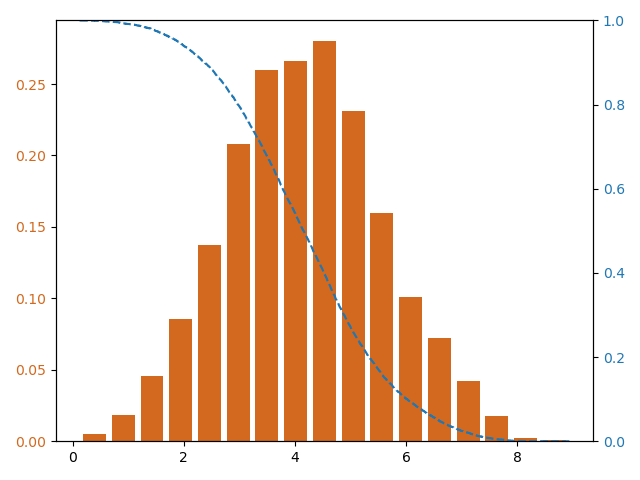
\includegraphics[width=\columnwidth]{Figures/dataset_histogram.png}
	\caption{
        Histogram of the tip errors $e_p(L_3)$ after calibration. Orange bars indicate the density while the blue line represents the empirical CCDF. Calibration on $10,000$ random data points resulted in a mean of $4.172 \pm 1.394$ \si{mm} and a median of $4.155$ \si{mm}.
    }
    \label{fig:pos_err_distribution}
\end{figure}

To evaluate the model's performance and ensure correctness, the CTCR model used for data collection was based on the robot parameters used by Grassmann et al. \cite{GrassmanChenLiangBurgner-Kahrs_IROS_2022}.
The authors used an \textsc{Aurora} v2 electromagnetic tracking system to collect a dataset of $100,000$ robot configurations, including position vectors and quaternions for the distal ends, $L_\text{base}$, $L_3$, $L_2$, and $L_1$ in the tracking system's reference frame.
The dataset is available under an open license.
The robot's parameters (Table ~\ref{tab:robot_parameters}) were calibrated by solving a non-linear least squares problem using $10,000$ randomly selected data points.
An offset vector $\boldsymbol{\delta_p}$ was applied to the distal end positions to reduce sensor placement uncertainty, and these adjusted positions were then transformed to the robot's base frame.
The optimization function was specified as
\begin{align*}
    & \boldsymbol{P} = \begin{bmatrix}
        \boldsymbol{\delta}_{p, L_\text{base}}^T & \boldsymbol{\delta}_{p, L_3}^T & \boldsymbol{\delta}_{p, L_2}^T & \boldsymbol{\delta}_{p, L_1}^T
    \end{bmatrix}^T \\
    & \boldsymbol{P}_{\text{optimal}} = \underset{\boldsymbol{P}}{\operatorname{argmin}} \left( e_{p}(L_1) + e_{p}(L_2) + e_{p}(L_3) \right)
\end{align*}
where $e_p = \|\boldsymbol{r}_{\text{model}}(s) - \boldsymbol{r}_{\text{data}}(s) \|_2$.
Calibration was performed using the Trust Region Reflective (TRF) algorithm via \textsc{Scipy}'s \texttt{optimize.least\_squares} function.

\begin{table}[thb!]
	%\vspace*{-4mm}
	\centering
	\caption{Tube Parameters of the CTCR from \cite{GrassmanChenLiangBurgner-Kahrs_IROS_2022}.}
	\label{tab:robot_parameters}
	\begin{tabular}{@{} lll r r r @{}}
		\toprule
		\multicolumn{3}{c}{Parameter}
		& \multicolumn{3}{c}{Tubes$^1$}\\
		\cmidrule(r){1-3}
		\cmidrule(l){4-6}
		\multicolumn{1}{c}{Term}
		& \multicolumn{1}{c}{Symbol}
		& \multicolumn{1}{c}{Unit}
		& \multicolumn{1}{c}{inner}
		& \multicolumn{1}{c}{middle}
		& \multicolumn{1}{c}{outer}\\
		\cmidrule(r){1-1}
		\cmidrule(lr){2-2}
		\cmidrule(lr){3-3}
		\cmidrule(lr){4-4}
		\cmidrule(lr){5-5}
		\cmidrule(l){6-6}
	    Length, overall		    & $L$				& \si{mm} 		& \num{210} 	&    \num{165} 	&     \num{110} 	\\
	    Length, straight	    & $L_\mathrm{s}$	& \si{mm} 		& \num{41} 	&    \num{100} 	&     \num{100} 		\\
	    Curvature$^2$ 			& $\kappa_x$		& \si{m}$^{-1}$ 	& \num{28} 	&    \num{12.4} &     \num{4.37}	\\
	    Diameter, outer$^2$		& $d_\text{outer}$	& \si{mm} 		& \num{0.5} 	&    \num{0.9} 	&     \num{1.5}		\\
	    Diameter, inner$^2$		& $d_\text{inner}$	& \si{mm} 		& \num{0.4} 	&    \num{0.7} 	&     \num{1.2}		\\
	    Young's Modulus		    & $E$				& \si{GPa} 		& \num{50} 		&    \num{50} 	&     \num{50} 		\\
	    Poisson's ratio		    & $\nu$				& \num{1} 		& \num{0,3} 	&    \num{0,3} 	&     \num{0,3}		\\
		\bottomrule
	\end{tabular}
	\hspace*{5mm}
	\begin{enumerate}
		\item[$^1$]\hspace{-2.5mm} The inner, middle, and outer tubes are referenced to 1, 2, and 3, respectively.
		\item[$^2$]\hspace{-2.5mm} The tube diameters and curvature are taken from the manufacturer's data sheet.
	\end{enumerate}
\end{table}
}


\bulletpoints{
    \item Topic Sentence: Discuss the results of the calibration and how it compares to the literature
    \item What is the average position error?
    \item Is the data obtained consistent with the literature?
    \item How can these results be improved?
}

\commentblock{

The average tip position error was $4.172$ \si{mm} which is $1.99\%$ of the total arc length.
Approximately $92.7\%$ of the tip errors were below $6.3$ \si{mm}, or $3\%$ of the total arc length, which is consistent with the literature \cite{Burgner-Kahrs_TRO_2015, Gilbert_Springer_2016}.
Further fine-tuning of the position error can be achieved by calibrating the stiffness matrix values, as discussed in \cite{RuckerJonesWebster_TRO_2010}.

\begin{table}[H]
	\centering
	\caption{Values of Calibrated Parameters}
	\label{tab:lst_sqrs}
	\begin{tabular}{l r r r}
		\toprule
		\multicolumn{1}{c}{Tube End}
		& \multicolumn{1}{c}{$\delta x$ in \si{mm}}
		& \multicolumn{1}{c}{$\delta y$ in \si{mm}}
		& \multicolumn{1}{c}{$\delta z$ in \si{mm}} \\
		\cmidrule(r){1-1}
		\cmidrule(lr){2-2}
		\cmidrule(lr){3-3}
		\cmidrule(lr){4-4}
	    $L_\text{base}$ & \num{2.179} & \num{11.264} & \num{1.006} \\
	    $L_3$ & \num{1.844} & \num{-0.184} & \num{0.504} \\
	    $L_2$ & \num{-0.523} & \num{-4.690} & \num{-1.321} \\
	    $L_1$ & \num{-3.501} & \num{-6.389} & \num{-0.177} \\
		\bottomrule
	\end{tabular}
\end{table}

\begin{table*}
	\centering
	\caption{Average Performance of Different Numerical Models}
	\label{tab:results}
	\begin{tabular}{r rrrr rrrr rrrr}
		\toprule
		& \multicolumn{4}{c}{Newton -- Rotation Matrix}
		& \multicolumn{4}{c}{Broyden -- Rotation Matrix}
        & \multicolumn{4}{c}{Broyden -- Quaternion}\\
		\cmidrule(lr){2-5}
		\cmidrule(lr){6-9}
		\cmidrule(l){10-13}
		\multicolumn{1}{c}{\hfill  Integrator}
		& \multicolumn{1}{c}{$e_p$ in \si{mm}}
		& \multicolumn{1}{c}{$n_{\boldsymbol{f}}$}
		& \multicolumn{1}{c}{$k$}
		& \multicolumn{1}{c}{$t$ in $\mu$\si{s}}
		& \multicolumn{1}{c}{$e_p$ in \si{mm}}
		& \multicolumn{1}{c}{$n_{\boldsymbol{f}}$}
		& \multicolumn{1}{c}{$k$}
		& \multicolumn{1}{c}{$t$ in $\mu$\si{s}}
		& \multicolumn{1}{c}{$e_p$ in \si{mm}}
		& \multicolumn{1}{c}{$n_{\boldsymbol{f}}$}
		& \multicolumn{1}{c}{$k$}
		& \multicolumn{1}{c}{$t$ in \si{\mu s}}\\
		\cmidrule(r){1-1}
		\cmidrule(lr){2-2}
		\cmidrule(lr){3-3}
		\cmidrule(lr){4-4}
		\cmidrule(lr){5-5}
		\cmidrule(lr){6-6}
		\cmidrule(lr){7-7}
		\cmidrule(lr){8-8}
		\cmidrule(lr){9-9}
		\cmidrule(lr){10-10}
		\cmidrule(lr){11-11}
		\cmidrule(lr){12-12}
		\cmidrule(l){13-13}
    FE              & $2.302$ & $1790$ & $4.36$ & $\mathbf{305}$ 
                    & $2.302$ & $963$  & $\mathbf{5.12}$ & $\mathbf{164}$
                    & $2.229$ & $\mathbf{963}$  & $5.13$ & $\mathbf{155}$ \\
    AB 2	        & $2.041$ & $\mathbf{1787}$ & $\mathbf{4.35}$ & $327$  
                    & $2.039$ & $\mathbf{962}$  & $\mathbf{5.12}$ & $184$ 
                    & $2.037$ & $\mathbf{963}$  & $5.13$ & $172$ \\
    AB 3      	    & $2.034$ & $1788$ & $\mathbf{4.35}$ & $348$ 
                    & $2.034$ & $963$  & $5.13$ & $191$ 
                    & $2.028$ & $\mathbf{963}$  & $5.13$ & $182$ \\
    AB 4        	& $2.035$ & $1790$ & $4.36$ & $374$ 
                    & $2.035$ & $963$  & $\mathbf{5.12}$ & $204$ 
                    & $2.029$ & $\mathbf{963}$  & $5.13$ & $200$ \\
    AB 5        	& $2.035$ & $1789$ & $\mathbf{4.35}$ & $405$ 
                    & $2.035$ & $964$  & $5.13$ & $217$ 
                    & $2.028$ & $\mathbf{963}$  & $5.13$ & $212$ \\
    RK 2        	& $2.027$ & $3575$ & $\mathbf{4.35}$ & $537$ 
                    & $2.027$ & $1924$ & $5.13$ & $292$ 
                    & $\mathbf{2.025}$ & $1925$ & $\mathbf{5.12}$ & $288$ \\
    RK 3        	& $2.025$ & $5366$ & $4.36$ & $785$ 
                    & $\mathbf{2.025}$ & $2889$ & $5.13$ & $426$ 
                    & $\mathbf{2.025}$ & $2887$ & $5.13$ & $413$ \\
    RK 4        	& $\mathbf{2.024}$ & $7151$ & $\mathbf{4.35}$ & $1032$ 
                    & $\mathbf{2.025}$ & $3851$ & $5.13$ & $558$ 
                    & $\mathbf{2.025}$ & $3847$ & $\mathbf{5.12}$ & $541$ \\

		\bottomrule
	\end{tabular}
	%https://tex.stackexchange.com/questions/112343/beautiful-table-samples
\end{table*}
}

\subsection{Computational Benchmark}

\bulletpoints{
    \item Topic Sentence: The benchmark used to evaluate the level of optimization is the number of function calls and runtime. This is because this combination captures minute improvements and is easier to work with.
    \item Function calls will be the benchmark along with runtime
    \item The other methods of assessing computational complexity are flawed due to their failure of capturing intricate interactions (e.g. quaternion constant runtime improvement).
    \item Butter up the reader and tell him that we are using a practical metric.
}

\commentblock{
In this paper, the primary benchmark for measuring computational complexity will be a combination of the number of function calls to $\boldsymbol{f}(s, \boldsymbol{y})$ and computational runtime.
While other methods, such as asymptotic complexity analysis and runtime measurements alone, have their merits, they often fall short in capturing the intricate interactions involved in optimization, such as constant runtime improvements due to quaternion representation.
By focusing on function call count and runtime, we provide a more accurate and accessible metric that directly reflects the optimization level achieved.
}

\subsection{Results}

\bulletpoints{
    \item Topic Sentence: Compare and contrast the performance of the different solvers.
    \item 99.8\% of all sample configurations converged successfully. The position error between Newton and Broyden was non-existent
    \item The broyden update reduced the number of function calls by 54\%
    \item The difference in accuracy between RK and AB methods is 16 micrometers, making it negligible for practical purposes.
    \item Using quaternion rotations lowered the error slightly and lowered runtime by 5\%
}

\commentblock{
Across all model types, the iteration count remained relatively low with $99.8\%$ of all sampled configurations converging successfully.
The position error was virtually identical between Newton and Broyden non-linear solvers; nonetheless, the Broyden update method reduced function calls by about $54\%$.
Although using RK integrators resulted in a slightly more accurate solution when compared to AB methods, the difference in the position error was \SI{16}{\mu m} on average making it negligible for practical purposes.
With a $5\%$ reduction in runtime and no change in function calls, the quaternion-based model offers improved stability during integration, highlighting the importance of constant runtime improvements for enhancing overall efficiency.
}

\bulletpoints{
    \item Topic Sentence: Compare and contrast the performance of the integrators. 
    \item AB integrator lowers function call count by 75\% while only increasing error by 0.8\%.
    \item FE only increase the position error by 0.278 mm compared to RK4.
    \item The optimal h for jacobian initialization is 7 mm.
    \item The approximation achieves a $25\%$ reduction in number of function calls with no effect on error.
}

\commentblock{
Using the second-order AB integrator instead of the fourth-order RK method leads to a $75\%$ reduction in function calls with only a $0.8\%$ increase in position error.
Although FE resulted in the highest position error across all integrators, the difference in position error between it an fourth-order RK is only \SI{0.278}{mm} or $0.1\%$ of the CTCR's arc-length, making it sufficient for practical use unless high accuracy is essential.
To determine the appropriate level of estimation for initializing the inverse Jacobian, a variety of $h_\text{initial}$ were examined using the Broyden model with FE and quaternion integration.
For this specific CTCR parameter set, the optimal $h_\text{initial}$ appears to be around \SI{7}{mm}, achieving a $25\%$ reduction in the number of function calls with no effect on the model's accuracy (Table~\ref{tab:h_step}).

\begin{table}[H]
	\centering
	\caption{Performance of Various $h_\text{initial}$ Values.}
	\label{tab:h_step}
	\begin{tabular}{l r r r r}
		\toprule
		\multicolumn{1}{c}{$h_\text{initial}$ in \si{mm}}
		& \multicolumn{1}{c}{$e_p$ in \si{mm}}
		& \multicolumn{1}{c}{$n_f$}
		& \multicolumn{1}{c}{$k$}
		& \multicolumn{1}{c}{$t$ in \si{\mu s}}\\
		\cmidrule(r){1-1}
		\cmidrule(lr){2-2}
		\cmidrule(lr){3-3}
		\cmidrule(lr){4-4}
		\cmidrule(l){5-5}
	    $3$ & $\mathbf{2.228}$ & $753$ & $\mathbf{5.79}$ & $124$ \\
        $4$ & $\mathbf{2.228}$ & $735$ & $5.95$ & $122$ \\
        $5$ & $2.230$ & $729$ & $6.09$ & $121$ \\
        $6$ & $2.229$ & $727$ & $6.20$ & $121$ \\
        $7$ & $\mathbf{2.228}$ & $\mathbf{726}$ & $6.30$ & $\mathbf{120}$ \\
        $8$ & $\mathbf{2.228}$ & $729$ & $6.39$ & $121$ \\
		\bottomrule
	\end{tabular}
\end{table}
}
